\cotefile{136}
\scanpage{111}
\begin{center}Foncteurs de De Rham généralisés\end{center}
On s'intéresse aux foncteurs
\[
 C^{**}:(\mathrm{Ss})^{o}\longrightarrow
 \left[\begin{aligned}
 &S_k\text{-algèbres bigraduées \inserted{alternées}}\\
 &\text{différentielles homogènes}\\
 &\text{\unsure{ties|tées} à p.d. (bidegrés}\\
 &\text{positifs, diff. de degré}\\
 &+1,\ \ldots\ldots\,)
 \end{aligned}\right]=\unsure{\mathscr S_k\mathscr D|S_k\mathscr D|\mathfrak D}
\]
\margin{$\unsure{o|\circ}$}
et on s'intéresse à ceux qui transforment $\underrightarrow{\lim}$ quelconques de $\mathrm{Ss}$ en $\underleftarrow{\lim}$, donc qui sont représentables.
Ils \deleted{\unsure{doivent|donnent}} \inserted{peuvent} donc s'interpréter \inserted{(\unsure{fonctoriellement|ponctuellement|fantasmes})} comme des $S_k$-algèbres bigraduées alternées \ldots\ $1/2$ simpliciales, i.e. des foncteurs
\[
 \mathbb{\Delta}^{o}\longrightarrow\mathscr D
\]
où on identifie dans les notations les deux sortes d'objets, écrivant \unsure{en|un}
\[
 C^{**}=C_*^{**}=(C_n^{**})_{n\geq 0}\quad\ldots
\]
et de $=$ pour les morphismes entre foncteurs, correspondant aux morphismes entre ensembles $1/2$ simpliciaux, respectant toutes les structures.

À $C_*^{**}$ est associé un foncteur ``cohomologie de De Rham associée à $C_{\unsure{*}}^{**}$''
\[
 \mathscr H_C^{**}(\mathscr X)=H_{\unsure{\mathscr S|\mathrm{gr}|\mathrm{G}|\varepsilon}}^{**}(C^{**}(\mathscr X))
\]
à valeurs dans les $S_k$-algèbres bigraduées alternées. On s'intéresse aux $C^{**}\deleted{(\mathscr X)}$ (dits admissibles) pour lesquels, pour tt $\mathscr X$,
% archive sheet number: 110
\scanpage{112}
\mspage{- 123 -}\hfill IX

et par passage aux modèles de Néron définit donc un homomorphisme sur les tores maximaux des fibres spéciales, donc en sens inverse un homomorphisme sur les Groupes de caractères, d'où un homomorphisme
\[
 \xi_t:\overline M\longrightarrow\underline M'\quad,\tag*{(10.2.6)}
\]
où $\overline M$ est défini en termes de $\overline A_K$ comme $\underline M$ en termes de $A_K$. On peut donc former l'accouplement
\[
 \varphi^t_\xi:\underline M_\ell\otimes\underline{\overline M}_\ell\longrightarrow\mathbb Z_\ell
 \quad,\quad\varphi^t(x,y)=\varphi^t(x,\xi_t(y))\quad.\tag*{(10.2.7)}
\]
Notons en passant que pour un schéma abélien $A_K$ a réduction semi-stable variable, le Groupe constant tordu $\underline M$ est un foncteur covariant en $A_K$, et qu'alors la formation des accouplements (10.2.7) associés aux biextensions de schémas abéliens à réduction semi-stable sur $(K,S)$ est compatible, en un sens évident, avec la formation des images inverses de biextensions. Bien entendu, lorsque $\xi$ est la biextension canonique ( ``de Weil'' ) de $(A_K,A'_K)$, l'accouplement (10.2.7) n'est autre que l'accouplement de monodromie (9.2.1). - Ceci posé, la relation de symétrie peut s'exprimer de la façon suivante : considérons la symétrique $ {}^s\xi$ de $\xi$, qui est une biextension de $(\overline A_K,A_K)$, d'où un accouplement
\[
 \varphi^t_{{}^s\xi}:\underline{\overline M}_\ell\otimes\underline M_\ell\longrightarrow\mathbb Z_\ell\quad;
\]
on a alors la relation de symétrie
\[
 \varphi^t_{{}^s\xi}=\varphi^t_\xi\circ s\quad,\quad\text{où}\quad
 s:\underline{\overline M}_\ell\otimes\underline M_\ell\xrightarrow{\sim}\underline M_\ell\otimes\underline{\overline M}_\ell
 \tag*{(10.2.8)}
\]
est encore l'isomorphisme de symétrie. On comparera cette relation à la relation d'antisymétrie de VIII 2.2.11.

\mspage{\handwritten{441}}
% stamp: numbered label 441
% archive sheet number: 111
\scanpage{113}
$\tau_\omega(H^{**}(\mathscr X))$ [qui est une algèbre graduée \deleted{\unsure{asso}} alternée, entre autres, de $M_\omega$] est \deleted{provient d'un} dans l'image essentielle de $\mathrm{Mod}(k)$, i.e. peut s'écrire (de façon ess. unique \unsure{à} $\unsure{\cong}$ \unsure{au niveau module|ou encore usuelle})
\[
 \mathscr H_C^{**}(\mathscr X)=\deleted{H}\!H_C^*(X)\otimes_k S_k
\]
[ et on sait que $H_C^*(X)$ hérite alors la structure de $\unsure{k'|k|l'}$-algèbre graduée de $\tau_\omega(H^{**}(\mathscr X))$. Cela implique que \deleted{pour} les $\deleted{\unsure{A}}C_n^{**}$ ont la $=$ propriété (faire $\mathscr X=\Delta_n$).
\deleted{On veut de plus que \inserted{$\forall\mathscr X$,} l'augmentation $S_k\to C^{**}(\mathscr X)$ définisse} On va préciser cette exigence

On peut considérer $\deleted{\unsure{A}}C_n^{**}$ comme un faisceau (à structure de type $\mathscr D$) sur \deleted{\unsure{la}} le topos $(\mathrm{Ss})$, il est coaugmenté par le faisceau constant $S_k$
\[
 S_k\longrightarrow C_{n}^{**}
\]
\deleted{\unsure{d'où}} [NB, on regarde ici le degré extérieur comme degré principal] de sorte qu'on a un diagramme (dans \deleted{\unsure{la}} cat. dérivée \deleted{$D(S_k$} \deleted{\unsure{consistant d'objets}} \inserted{$D(S_k\text{-mod gradué})$}) :
\diagram{\begin{tikzcd}[ampersand replacement=\&,column sep=small]
 \mathbb R\Gamma^{\unsure{*}}(\mathscr X,S_k)\arrow[r] \& \mathbb R^{*}\Gamma(\mathscr X,C_{\unsure{*|n}}^{**})\\
 |[alias=tag]|{\text{(1)}} \& C^{**}(\mathscr X)=\Gamma(\mathscr X,C^{**}\arrow[u]
\end{tikzcd}}
% archive sheet number: 112
\scanpage{114}
\mspage{- 122 -}\hfill IX
\[
 u_\ell^{A'_K}=u_\ell^{A_K}\,s\quad.\tag*{(10.2.2)}
\]

Compte tenu de la propriété connue d'anticommutativité des accouplements $\varphi_\xi$ ([5] ou VIII 2.2.11), la formule de symétrie (10.2.2) peut se reformuler de la façon suivante, en termes d'une polarisation fixée $\xi$ de $A_K$, qui définit un homomorphisme $\widetilde\xi:A_K\longrightarrow A'_K$, d'où un homomorphisme correspondant ($t$ étant l'initiale de ``torique'')
\[
 \xi_t:\underline M\longrightarrow\underline M'\quad,\tag*{(10.2.3)}
\]
permettant de former l'accouplement
\[
 \varphi^t_{\xi\ell}:\underline M_\ell\otimes\underline M_\ell\longrightarrow\mathbb Z_\ell
 \ ,\ \varphi^t_{\xi,\ell}(x,y)=u_\ell^{A_K}(x,\xi_t(y))\quad:\tag*{(10.2.4)}
\]
la forme précédente $\varphi^t_{\xi,\ell}$ est \uline{symétrique} :
\[
 \varphi^t_{\xi\ell}(x,y)=\varphi^t_{\xi\ell}(y,x)\quad.\tag*{(10.2.5)}
\]
En fait, cet énoncé est valable pour tout élément $\xi$ du groupe de Néron-Séveri de $A_K$ (pas nécessairement une polarisation) ; mais ce n'est que lorsque $\xi$ est non dégénéré i.e. définit une \uline{isogénie} $A_K\to A'_K$ donc aussi une isogénie (10.2.3), que la relation de symétrie (10.2.5) est équivalente à la relation de symétrie (10.2.2). D'ailleurs dans le cas où $\xi$ est une polarisation, on va préciser considérablement (10.2.5) dans 10.4 b) plus bas.

Signalons enfin une troisième façon d'interpréter la relation de symétrie. Pour ceci, considérons une biextension (= correspondance divisorielle) $\xi$ sur un couple $(A_K,\overline A_K)$ de schémas abéliens à réduction semi-stable sur $K$, qui définit un homomorphisme
\[
 A_K\longrightarrow\overline A'_K\quad,
\]
\mspage{\handwritten{440}}
% stamp: numbered label 440
% archive sheet number: 113
\scanpage{115}
\deleted{En fait, on demande qu'}En appliquant $\tau_\omega\unsure{=|:|\simeq|\text{à}}\mathbb R^*\tau_\omega$, on trouve
\diagram{\(\text{(2)}\quad\)\begin{tikzcd}[ampersand replacement=\&,column sep=small]
 \deleted{\mathbb R^*}\tau_\omega(\mathbb R^*\Gamma(\mathscr X,S_k))\arrow[r] \& \deleted{\unsure{\mathbb R^*}}\tau_\omega\mathbb R^*\Gamma(\mathscr X,C^{**}).\\
 \& \tau_\omega C^{**}(\mathscr X)\arrow[u]
\end{tikzcd}}
On \deleted{demande} \inserted{voudrait} que ces deux flèches soient des isomorphismes \inserted{dans la cat. dérivée}, ce qui signifie aussi que les hom. déduits de (1) en passant à la coh.
\diagram{\(\text{(1$'$)}\quad\)\begin{tikzcd}[ampersand replacement=\&]
 H^{**}(\mathscr X,S_k)\arrow[r] \& H^{**}(\mathscr X,C^{**})\\
 \&\mathscr H_C^{**}(X)\arrow[u]
\end{tikzcd}}
soient à noyau et conoyau négligeables, ce qui \deleted{signifie} \inserted{implique} précisément, pour la flèche horizontale, qu'on a
\diagram{\(\displaystyle (\deleted{\unsure{1}}2')\left\{\vcenter{\hbox{\begin{tikzcd}[ampersand replacement=\&,column sep=small]
 \tau_\omega(\deleted{\unsure{t}}H^*(\mathscr X,k)\otimes_k S_k)\arrow[r,"\sim"]\arrow[dr,dashed,no head] \& \tau_\omega \mathbb H^{**}(\mathscr X,C^{**})\\
 \&\tau_\omega(\mathbb H_C^{**}(\unsure{X|x}))\arrow[u,"\unsure{\wr|2}"']
\end{tikzcd}}}\right.\) }
% archive sheet number: 114
\scanpage{116}
\mspage{- 121 -}\hfill IX

10. \uline{Propriétés de l'accouplement de monodromie}. \uline{Théorème d'intégrité et de positivité}\unsure{.}

Dans le présent paragraphe, nous allons donner tout d'abord certaines propriétés formelles essentiellement triviales des accouplements de monodromie, le détail (un peu fastidieux) des vérifications étant laissé au lecteur. D'autre part, nous indiquons un théorème plus profond (10.4) concernant ces accouplements, et indiquons comment on peut se réduire pour sa démonstration à un cas spécial de jacobiennes, qui sera traité (par voie transcendante) au par. 12 (qui est d'ailleurs logiquement indépendant du par. 11).

10.1. \uline{Transport de structure}. Il est clair, sur la définition donnée de l'accouplement de monodromie (9.1.2), que cet accouplement est compatible avec le transport de structure en la situation $(S,A_K,A'_K)$.

10.2. \uline{Symétrie}. Si nous partons du schéma dual $A'_K$ de $A_K$ et lui appliquons la construction du par. 9, nous devons introduire le schéma dual $(A'_K)'$ de $A_K$, qui est canoniquement isomorphe à $A_K$ par le théorème de bidualité ([5] ou VIII 3.2). Désignons par $u_\ell^{A_K}$ l'accouplement de monodromie (9.1.2) relativement à $A_K$, de sorte qu'on trouve de même un accouplement
\[
 u_\ell^{A'_K}:\underline M'_\ell\otimes\underline M_\ell\longrightarrow\mathbb Z_\ell\quad.\tag*{(10.2.1)}
\]
Ceci posé, je dis que ce dernier se déduit de $u_\ell^{A_K}$ par la symétrie
\[
 s:\underline M_\ell\otimes\underline M'_\ell\xleftarrow{\sim}\underline M'_\ell\otimes\underline M_\ell\quad,
\]
i.e. on a la formule

\mspage{\handwritten{439}}
% stamp: numbered label 439
% archive sheet number: 115
\scanpage{117}
Prenons $\mathscr X=\Delta_n$, alors \deleted{\unsure{les|le}} le diagramme (1) devient
\diagram{\begin{tikzcd}[ampersand replacement=\&,column sep=small]
 \mathbb R^*\Gamma(\Delta_n,S_k)\simeq S_k\arrow[r] \& \mathbb R^*\Gamma(\Delta_n,C^{**}\unsure{]|)}=\deleted{\unsure{A}}C_n^{**}\\
 \& C^{**}(\Delta_n)=C_n^{**}\arrow[u,"{\mathrm{id}_{C_n^{**}}}"']
\end{tikzcd}}
et la condition énoncée se réduit à celle concernant la flèche horizontale, qui signifie aussi
\diagram{\(\text{(3)}\quad\)\begin{tikzcd}[ampersand replacement=\&,column sep=0pt]
 H_C^{**}(\Delta_n)={} \& H^{**}(C_n^{**}) \& \deleted{\text{est isom}}\unsure{k|*}\\
 \& S_k\arrow[u,"{\varepsilon\ \text{augmentation}}"'] \&
\end{tikzcd}}
l'augmentation est un quasi-iso i.e.
\[
 \begin{aligned}
 &\deleted{\unsure{k}}\deleted{\unsure{=}}\deleted{\unsure{B}}S_k^i\longrightarrow
 \underset{\substack{\Vert\\\operatorname{Ker}(C_n^{i,0}\mathbin{-}C_n^{i1}).}}{H^{i0}(C_n^{**})}
 \deleted{\unsure{\simeq}}\ \text{est un}\\
 &\text{iso pour }i\text{ grand }(i\geq\lambda(\unsure{+0|+{\infty}|0|n})\ \text{disons})
 \end{aligned}\tag*{3 a)}
\]
\[
 \begin{aligned}
 &\forall p>0,\qquad H^{ip}(C_n^{**})=0\ \text{pour }i\\
 &i\text{ grand (dépendant de }p),\ \text{soit}\\
 &H^{ip}(\deleted{\unsure{S}}C_n^{**})=0\quad\text{si}\quad i\geq\deleted{\unsure{g}}\lambda(p)
 \end{aligned}\tag*{3 b)}
\]
où on peut supposer $\lambda:\mathbb N^{*}\mathbin{\unsure{-|\to}}\mathbb N^{*}$ strictement croissante.

A priori, ce $\lambda=\lambda_n$ dépend du choix de $n$. On suspecte qu'il faut pouvoir prendre $\lambda$ indépendant de $n$ --
% archive sheet number: 116
\scanpage{118}
Liebe Gertrud,\\
\quad Von einer dreiwöch
% archive sheet number: 117
\scanpage{119}
dans ce cas la flèche horizontale sera bien un isomorphisme \deleted{\unsure{dans|donc}} après application de $\tau_\omega$\ldots\ En effet, \unsure{ch.que|chaque} $C_*^{i*}$ est une résolution de $(S_k^i)_*$ (dans $(\mathrm{Ss})$), jusqu'au degré $p$ si $i$ est assez grand p.r. à $p$, \unsure{donc}\ldots.

\deleted{On} Regardons la condition d'isomorphie (après application de $\tau$) pour la flèche verticale, elle \deleted{est satisfaite} est conséquence de la condition suivante (et sans doute équivalente)

% slanted
\margin{On peut \deleted{\unsure{peut-être}} affaiblir (4), en prenant ``flasque jusqu'en une \unsure{dimension|générateurs} donnée'' (du côté $\mathrm{Ss}$)}
(4) Pour tt $i\geq0$ considérer les \inserted{groupes $1/2$ simpl.} $C_*^{ip}$ $(p\geq0)$ et soit $\pi(i)$ le plus petit entier (s'il existe) tel que $C_*^{ip}$ ne soit pas flasque ($\pi(i)=+\infty$ sinon), \deleted{\unsure{ceci veut}} i.e. que son \uline{\unsure{hologie|homologie|faisceaux}} $1/2$ simpliciale \inserted{(pour $\partial$)} soit non nulle. On veut que $\pi(i)\longrightarrow+\infty$ quand $i\longrightarrow+\infty$.

\figure{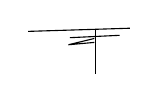
\begin{tikzpicture}[x=1cm,y=1cm]
 \draw (-.65,.18)--(.64,.22); \draw (.2,.20)--(.2,-.36);
 \draw (-.12,.1)--(.51,.13); \draw (.19,.09)--(-.14,.01)--(.19,.04);
\end{tikzpicture}}

On aimerait prouver un th. d'unicité (\unsure{ou.|ou} déjà l'existence\ldots)

Les $C_*^{**}$ ayant les structures précisées (au besoin en oubliant d'abord la structure p.d.) et satisfaisant
% archive sheet number: 118
\scanpage{120}
% letterhead
COLLÈGE\\
DE\\
FRANCE\\
\rule{1em}{.4pt}\\
\deleted{\textit{Paris, le}}xxxxx Massy le 14.9.1971\\
Cher Monsieur Poncet,\\
Je viens d'avoir connaissance de deux ennuis sérieux avec la machine Hermès 3000 que vous m'aviez livrée en juin: l\deleted{\unsure{a}}e margeur gauche ne fonctionne plus, et l'enroulement du ruban est défectueux, ne permettant d'utiliser qu'une partie du ruban et obligeant de ce fait à des manipulations supplémentaires fort gênantes. Ces ennuis se présentent alors que la machine a encore à peine servi (une trentaine de pages de texte environ), et il est clair que la qualité des machines Hermès 3000 a considérablement baissée depuis une dizaine d'années (j'ai une machine avec laquelle je n'ai eu aucun ennui depuis cette période). C'est pourquoi je me vois dans l'obligation \inserted{d'annuler} la commande d'une autre machine Hermès 3000 que je vous avais faite vers la fin du mois d'août (lettre datée erronnément du 1.6.1971 ...), préférant m'adresser à une marque de machine portative qui ne m'exposera pas à des contretemps continu\deleted{\unsure{le|el}}\unsure{el|le}s\unsure{.}

Au cas où à la réception de la présente lettre, la livraison aurait déjà été faite, je vous serais obligé de la reprendre au Collège de France. Je vous renvoie ci-joints facture et bon de garantie relatifs à cette commande.

Veuillez agréer, cher Monsieur, l'expression de ma considération\\
la plus distinguée\\
% archive sheet number: 119
\scanpage{121}
aux conditions supplémentaires techniques énoncées (être une ``quasi'' résolution de $S_k$, et être ``quasi-flasque''\ldots)

On note que les hom dans \deleted{\unsure{cette}} \inserted{la} catégorie des objets \inserted{$C_*^{**}$} envisagés sont déjà des ``quasi-isom'' (p.r. à $\tau_\omega$) -- il y a lieu de passer à la cat. des fractions en \deleted{les} rendant inversibles tous ces hom, \unsure{c.à} i.e. le groupoïde engendré par la catégorie envisagée. On aimerait donc prouver que ce groupoïde est connexe et simplement connexe ? [\uline{NB} rappelons que \unsure{ici} \uline{on ne bouge pas} \inserted{les \unsure{élts de|élémts de}} $S_k=k\{\unsure{T|t|\delta}\}$]

\inserted{Si on veut de plus qu'il y ait calcul des fractions à gauche,} Cela signifie donc

\margin{?}
\uline{Conj ?} a) Si $C_*^{**}$ et $C'_*{}^{**}$ sont des théories admissibles, $\exists$ théorie admissible $C''_*{}^{**}$ et hom
\diagram{\begin{tikzcd}[ampersand replacement=\&,row sep=small]
 \& C_*^{**}\\
 C''_*{}^{**}\arrow[ur]\arrow[dr,no head] \&\\
 \& C'_*{}^{**}
\end{tikzcd}}
% slanted
\margin{il y aurait plus de chances avec calcul de fractions à droite ???}
b) Si on a des hom
\diagram{\begin{tikzcd}[ampersand replacement=\&]
 \deleted{\unsure{S}}C'_*{}^{**}\arrow[r,shift left]\arrow[r,shift right] \& C_{*}^{**}
\end{tikzcd}}
$\exists$ hom
\[
 C''_*{}^{**}\mathbin{\unsure{-|\to}}C'_*{}^{**}
\]
qui ``égalise''.
% archive sheet number: 120
\scanpage{123}
\begin{flushright}\fbox{\shortstack{Complexes de \uline{\unsure{chaînes|chaines|duaux}} de De Rham\\à p.d.}}\end{flushright}
Soient

$k$ anneau comm

\deleted{$\unsure{S|A}$} \textcircled{$s$} une $k$-coalgèbre \inserted{ass. unitaire comm}

\deleted{\unsure{avec $k$}}
\[
 \boxed{s\longrightarrow s\otimes_k s}
\]
[donc \inserted{$V_k(\deleted{\unsure{S}}s):$} $k'\longmapsto s^{k'}=\operatorname{Hom}_k(s,k')$ est un foncteur à valeurs dans les anneaux ass. unit. comm, \unsure{soit|fait} une $\mathcal O_k$-Alg. ass. un. comm

\diagram{\begin{tikzcd}[ampersand replacement=\&,column sep=small]
 |[draw,circle,inner sep=1pt]|{\bar s}\arrow[d,shift left]\arrow[from=2-1,to=1-1,shift left] \& \text{une sous-}k\text{-coalgèbre \inserted{ass. unit. comm}}\\
 |[draw,circle,inner sep=1pt]|{s^+} \& {}=s/\bar s\quad\text{le }k\text{-module quotient}
\end{tikzcd}}
[donc \inserted{$V_k(\bar s):$} $k'\longmapsto\bar s^{k'}=\operatorname{Hom}_k(\bar s,k)$ est une $\mathcal O_k$-alg. ass. unit. comm et $s^{k'}\longrightarrow\bar s^{k'}$ est un hom de $k'$-Alg. ass. unit. comm \inserted{i.e. $V_k(s)\to V_k(\bar s)$ hom de $\mathcal O_k$-algs.}

[c'est une coalgèbre ass. comm mais pas unitaire]

[$s^{+\,k'}=\operatorname{Ker}(s^{k'}\to\bar s^{k'})\subset s^{k'}$ est un idéal de $s^{k'}$, donc $V_k(s^+)\overset{\text{déf}}=V_k(s)^+$ est un Idéal de $V_k(s)$]

\textcircled{$\gamma_*$} un système de copuissances divisées sur $(s,s^+)$

[donc on a sur $V_k(s^+)=V_k(s)^+$ un syst. de puiss. divisées
\[
 \gamma_i:V_k(s^+)\longrightarrow V_k(s^+),\quad i\geq1
\]
défini par des hom de $k$-alg
\[
 \gamma_i^*:\operatorname{Sym}_k(s^+)\longrightarrow\operatorname{Sym}_k^*(s^+)
\]
\deleted{\unsure{qui}} i.e. hom $k$-\unsure{lin|lin.}
\[
 \gamma_i^*:s^+\longrightarrow\operatorname{Sym}_k^*(s^+)
\]
qui, en vertu des axiomes sont en fait
\[
 \boxed{\gamma_i^*:s^+\longrightarrow\operatorname{Sym}_k^i(s^+)\quad(i\geq1)}
\]
avec des axiomes \unsure{dessus|divers}

$t:s^+\to k$ un $k$ hom \qquad i.e. $t\in V_k(s^+)(k)=V_k(s)^+(k)$

Alors on définit un objet simplicial dans la \unsure{cat.} des foncteurs
\[
 (k\text{-alg comm})\longrightarrow
 \left(\begin{aligned}
 &\text{algèbres graduées}\\[-2pt]
 &\text{alternées différentielles}\\
 &\text{(diff. de degré }+1)\text{ à}\\
 &\inserted{\text{avec idéal à}}\text{ puiss. divisées }\unsure{(|)}
 \end{aligned}\right.
\]
et $=$ dans la \unsure{cat.} des \deleted{foncteurs} schémas affines \deleted{$\unsure{S}$} en algèbres graduées alternées différentielles (diff. de degré $+1$) avec Idéal \inserted{homogène} à \unsure{puiss.|puissances divisées} (qui est un schéma affine), les puiss. divisées étant compatibles aux graduations et à la différentielle
% archive sheet number: 122
\scanpage{124}
\mspage{- 120 -}\hfill IX

un accouplement
\[
 v_\ell^{K'}:\underline M_K\otimes\underline M'_K\longrightarrow\mathbb Z_{\ell K}\quad.\tag*{(*)}
\]

Ce dernier à priori dépend du choix de $K'$, mais il résulte de (10.4.3) ci-dessous que l'accouplement
\[
 u_\ell:\underline M_K\otimes\underline M'_K\longrightarrow\mathbb Q_{\ell K}\tag*{(9.7.1)}
\]
donné par
\[
 u_\ell=(1/e(S'/S))\,v_\ell^{K'}
\]
n'en dépend pas, où $e(S'/S)=\operatorname{long}(V'/\underline m V')$. On pourra appeler encore (9.7.1) l'\uline{accouplement de monodromie} pour le schéma abélien $A_K$ sur $K$ et le nombre premier $\ell$ envisagé, puisque dans le cas où $A_K$ lui-même a réduction semi-stable, il coïncide évidemment avec la restriction à $\eta$ de l'accouplement de monodromie (9.1.2). Il résulte de 10.4 plus bas que cet accouplement est en fait toujours à valeurs dans $\mathbb Q_K$, et est indépendant de $\ell$.

On peut se demander s'il est à valeurs dans $\mathbb Z_K$, ce qui revient à dire que (9.7.1) est à valeurs dans $\mathbb Z_{\ell K}$ pour tout nombre premier $\ell$. C'est le cas du moins si $A_K$ est une courbe elliptique, le seul cas qui demande une vérification étant alors celui où $\underline M_K\simeq\underline M'_K$ est de rang 1, de sorte que $\underline M_K\otimes\underline M'_K$ est canoniquement isomorphe à $\mathbb Z_K$, et que l'accouplement de monodromie (9.7.1) peut s'interprèter simplement comme un nombre rationnel ordinaire. On trouve grâce aux résultats de NERON [19] que celui-ci est égal à $v(j)$, $j$ étant l'invariant absolu de $A_K$ et $v$ la valuation normalisée de $K$.

\mspage{\handwritten{438}}
% stamp: numbered label 438
% archive sheet number: 123
\scanpage{125}
\[
 \underbrace{\unsure{A|\mathscr A|\mathcal A}_*^*(\deleted{\unsure{S}}s,s^+,\gamma_*,t)}_{\substack{\text{schéma affine}\\\text{en alg. graduées}\\\text{(alternées) différentielles}\\\text{(}d\text{ de degré }\unsure{=|+}1)\ \text{avec idéal hom.}\\\text{à p.d. (\unsure{ce qu'on veut|comp. au reste})}}}(k')
 =A_*^*\bigl(\underset{\substack{\Vert\\V_k(s)(k')}}{s^{k'}},
 \underset{\substack{\Vert\\V_k(s^+)(k')}}{(s^{k'})^+},\gamma_*^{k'},t^{\unsure{k'|k}}\bigr)
\]
On a
\[
 A_*(s,s^+,\gamma_*,t)(k')(\bar I)
 \simeq \widehat{\unsure{\Gamma|\Pi}}_{s^{k'}\deleted{\unsure{*}}}^{\unsure{\prime|*}}\{\{\,k'^{I}\}\}
 \otimes_{k'}\Lambda^*(k'^{I}\deleted{\unsure{1}}/k')\big/
 \substack{\text{idéal}\\\text{p.d.}\\\text{engendré}\\\text{par }\sum X_i-t}
\]
\[
\begin{aligned}
 A_n(s,s^+,\gamma_*,t)(k')&\simeq\deleted{\unsure{k}}s^{k'}\{\{X_0,\ldots,\overset{\substack{\inserted{\unsure{\simeq}\Gamma}\\\nearrow}}{X_n}\}\}
 [dX_0,\ldots,dX_n]/(\textstyle\sum X_i-t,\sum dX_i)_{\mathrm{pd}}\\
 &\simeq s^{k'}\{\{X_0,\ldots,X_{n-1}\}\}[dX_0,\ldots,dX_{n-1}]\\
 &\underset{\substack{\text{comme}\\\text{foncteur en}\\k'}}{\simeq}
 \deleted{\unsure{k|\prod}}(s^{k'})^{\mathbb N^n\times\underset{\text{\inserted{ens des parties}}}{\unsure{\mathcal P|\mathfrak P}}([0,n-1])}\\
 &\underset{\substack{\text{comme foncteur en}\\ k'}}{\simeq}
 \operatorname{Hom}_k(s,k')^{\mathbb N^n\times\mathcal P([0,n-1])}\\
 &\underset{\ldots}{\simeq}\operatorname{Hom}_k\bigl(s^{(\mathbb N^n\times\mathcal P(\,[0,n-1]) )},k'\bigr)\\
 &= V\bigl(\underbrace{s^{(\mathbb N^n\times\mathcal P([0,n-1]))}}_{\vphantom{X}}\bigr)(k')\\
 &= V\bigl(s\otimes_k k[Y_0,\ldots,Y_{n-1}]\otimes_k\Lambda^*(y_0,\ldots,y_{n-1})\bigr)(k')
\end{aligned}
\]
\[
 A_n(s,s^+,\gamma_*,t)(k')/A_n(\qquad)(k')^+
 \simeq s^{k'}/(s^{k'})^+\longleftarrow\bar s^{k'}
\]
\diagram{\begin{tikzcd}[ampersand replacement=\&,column sep=small,row sep=small]
 A_n(\qquad)(k')\arrow[r]\arrow[d,equal] \& \bar s^{k'}=V(\bar s)(k')\\
 V(s\otimes_k k[Y_0,\ldots,Y_{n-1}]\otimes_k\Lambda^{\unsure{*|2}}(y_0,\ldots,y_{n-1}))(k')\arrow[r] \& V(\bar s)(k')
\end{tikzcd}}
\diagram{\begin{tikzcd}[ampersand replacement=\&,column sep=small,row sep=small]
 s\otimes_k k[Y_0,\ldots,Y_{n-1}]\otimes_k\Lambda^*(y_0,\ldots,y_{n-1}) \& \& \bar s\arrow[ll]\arrow[dl,hook]\\
 \& s\arrow[ul,hook] \&
\end{tikzcd}}
On voit donc, posant
\[
 A_{*}^n(s,s^+,\gamma_*,t)=s\otimes_k k[Y_0,\ldots,Y_{n-1}]\otimes_k\Lambda^*(y_0,\ldots,y_{n-1})
\]
% archive sheet number: 124
\scanpage{126}
\mspage{- 119 \unsure{·|-}}
\hfill IX

Comme extension panachée $X_\eta$ de $E_\eta$ par $F_\eta$, on prendra
\[
X_\eta=T_\ell(A_K)=X_\eta^0\supset X_\eta^1=T_\ell(A_K)^f\supset X_\eta^2=T_\ell(A_K)^t\supset 0\quad . \tag*{(9.6.2)}
\]
L'isomorphisme d'extensions de $R_\eta$ par $P_\eta$
\[
X_\eta^1\simeq F_\eta
\]
est clair. L'isomorphisme d'extensions de $Q$ par $R$ :
\[
X_\eta/X_\eta^2\simeq F_\eta=D(F'_\eta)
\]
est clair grâce au théorème d'orthogonalité 5.2.

Nous disposons donc des données requises pour définir un accouplement (9.5.6)\textsuperscript{\handwritten{\unsure{x|$\times$}}}, qui ici (comme $Q*= \underline{M}'_\ell$) prend la forme (9.1.2). Le fait que cette définition soit compatible avec celle de 9.2 résulte de 9.5.8. Les considérations de 5.8 montrent d'autre part, sous réserve de la validité du théorème de TATE [33] (donc en tous cas dans le cas où $\mathrm{car}\ K=0$) que l'accouplement en question peut se décrire en termes du seul $\ell$-pro-groupe de Barsotti-Tate $X_\eta=T_\ell(A_K)$ sur $S$ (puisque sa filtration en trois crans, et les extensions $F$ et $E$ qui prolongent $X_\eta^1$ et $X_\eta/X_\eta^2$, peuvent se définir canoniquement en termes du seul pro-$\ell$-groupe $X=T_\ell(A_K)$.

\uline{Remarque} 9.7. Ne supposons plus nécessairement que $A_K$ ait réduction semi-stable sur le trait hensélien $S$, et soit $K'$ une extension galoisienne finie de $K$ telle que $A_{K'}$ ait réduction semi-stable sur le normalisé $S'$ de $S$ dans $K'$ (3.6). Avec les notations de (8.1.8), on définit alors, par descente galoisienne à partir de l'accouplement de monodromie pour $A_{K'}$,

\mspage{\handwritten{\unsure{437}}}
% stamp: numbered label 437
% archive sheet number: 125
